\documentclass[a4paper, 12pt]{article}%тип документа



%отступы
\usepackage[left=1cm,right=1cm,top=1cm,bottom=2cm,bindingoffset=0cm]{geometry}

%%% Работа с русским языком
\usepackage{graphicx}
\usepackage{cmap}                           % поиск в PDF
\usepackage{mathtext} 			 	       % русские буквы в формулах
\usepackage[T2A]{fontenc}               % кодировка
\usepackage[utf8]{inputenc}              % кодировка исходного текста
\usepackage[english,russian]{babel} 
\usepackage{float}
\usepackage{sidecap}
\usepackage{graphicx}
\usepackage{wrapfig}
\usepackage{multirow}
\usepackage[export]{adjustbox} % локализация и переносы
\usepackage[unicode, pdftex]{hyperref}
\usepackage{subfig}% http://ctan.org/pkg/subfig
\usepackage{booktabs}

\usepackage{wrapfig}


%Матеша
\usepackage{amsmath,amsfonts,amssymb,amsthm,mathtools} % AMS
\usepackage{icomma} % "Умная" запятая

%\mathtoolsset{showonlyrefs=true} % Показывать номера только у тех формул, на которые есть \eqref{} в тексте.

%% Шрифты
\usepackage{euscript}	 % Шрифт Евклид
\usepackage{mathrsfs} % Красивый матшрифт

%% Свои команды
\DeclareMathOperator{\sgn}{\mathop{sgn}}

%% Перенос знаков в формулах (по Львовскому)
\newcommand*{\hm}[1]{#1\nobreak\discretionary{}
	{\hbox{$\mathsurround=0pt #1$}}{}}
\newcommand{\rref}[1]{(\ref{#1})}
\newenvironment{comment}{}{}
\newcommand{\picref}[1]{рис. \ref{#1}}
\newcommand{\mbf}{\mathbf}
\newcommand{\Equip}[3]{
	
	{\bf #1:} $\Delta = \pm #2$ \si{#3}}
\newcommand{\equip}[1]{
	
	{\bf #1}}

%\usepackage{caption}
%\usepackage{subcaption}


\author{Гаврилин Илья Дмитриевич \\
	Б01-101}
\title{\textbf{Лабораторная работа 4.3.2\\ 
		Дифракция света на ультразвуковой волне в жидкости}}
	
\begin{document}
	\maketitle
	\section{Аннотация}
	В работе определили скорость звуковой волны в жидкости при помощи дифракционной картины. Также в качестве второго способа воспользовались методом темного поля.
	\section{Теоретические сведения}
	
	
	В работе используются оптическая скамья, осветитель, два длиннофокусных объектива, кювета с жидкостью, кварцевый излучатель с микрометрическим винтом, генератор звуковой частоты, линза, горизонтальная нить на рейтере, микроскоп. 
	
	При прохождении ультразвуковой волны через жидкость в ней возникают периодические неоднородности коэффициента преломления, создается фазовая решетка, которую мы считаем неподвижной ввиду малости скорости звука относительно скорости света. Показатель
	преломления n изменяется по закону:
	
	\begin{equation}\label{}
	n = n_0 (1 + m \cos \Omega x)
	\end{equation}
	
	Здесь $ \Omega = 2 \pi / \Lambda $ --- волновое число для ультразвуковой волны, $ m $ --- глубина модуляции $ n $ $ (m \ll 1 $).
	
	Положим фазу $ \phi $ колебаний световой волны на передней стенке кюветы равной нулю, тогда на задней поверхности она равна:
	
	\begin{equation}\label{}
	\phi  = k n L = \phi_0 (1 + m \cos \Omega x)
	\end{equation}
	
	Здесь $ L $ --- толщина жидкости в кювете, $ k = 2 \pi / \lambda $ --- волновое число для света.
	
	После прохождения через кювету световое поле есть совокупность плоских волн, распространяющихся под углами $ \theta $, соответствующими максимумам в дифракции Фраунгофера:
	
	\begin{equation}\label{}	
	\Lambda \sin \theta_m = m \lambda
	\end{equation}
	
	Этот эффект проиллюстрирован на рисунке 1.
	\begin{figure}[H]
	\centering	
	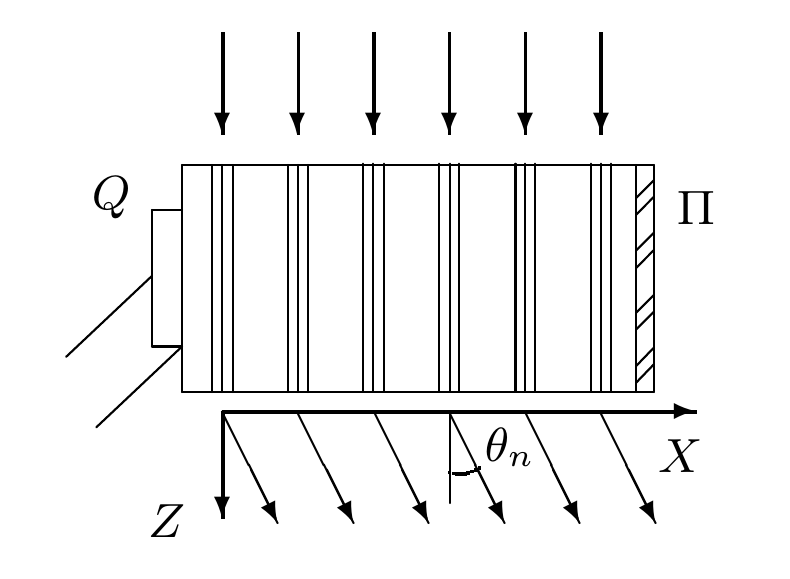
\includegraphics[width=0.3\linewidth]{difraction.png}
	\caption{Дифракция световых волн на акустической решетке}
	\label{fig:}
	\end{figure}
	
	Зная положение дифракционных максимумов, по формуле (1) легко определить длину ультразвуковой волны, учитывая малость $ \theta $: $ \sin \theta \approx \theta \approx l_m /F  $, где $ l_m $ --- расстояние от нулевого до последнего видимого максимума, $ F $ --- фокусное расстояние линзы. Тогда получим:
	
	\begin{equation}\label{}
	\Lambda = m \lambda F/ l_m 
	\end{equation}
	Скорость ультразвуковых волн в жидкости, где $ \nu $ --- частота колебаний излучателя:
	
	\begin{equation}\label{}
	v = \Lambda \nu 
	\end{equation}
	\section{Ход работы}
	\subsection{Определение скорости ультразвука по дифракционной картине}
	\begin{figure}[H]
		\centering
		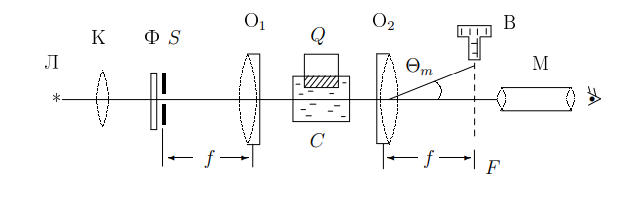
\includegraphics[width=0.8\linewidth]{shema1}
		\caption{Схема экспериментальной установки}
		\label{fig:shema1}
	\end{figure}
	Для получения картинки в данном случае на кювету с водой подается сигнал с ультразвукового излучателя, после с помощью подстройки частоты и положения излучателя в воде подбирается момент образования стоячей волны. В микроскоп наблюдаем дифракцию на данной акустической решетке.\\
	\textit{В ходе работы была замечена сильная нестабильность показаний генератора на частотах больше 3-4 МГц, также отсутствовала возможность полноценно сфокусироваться на нижней поверхности щели, ввиду чего пострадало качество получаемых дифракционных картин. Ввиду вышеперечисленного замеры проводились на частотах до 2 МГц, пока картинка была различима.}\\
	\textbf{Построим зависимости координаты минимума от его номера для различных частот.}\\
	\begin{table}[H]
		\centering
		\begin{tabular}{|c|c|c|c|c|}
			\hline
			n      & -1   & 0    & 1 & 2    \\ \hline
			x, мкм & 2.62 & 2.36 & 2 & 1.69 \\ \hline
		\end{tabular}
		\caption{Зависимость координаты от порядка минимума (f = 983.321 кГц)}
	\end{table}
	\begin{figure}[H]
		\centering
		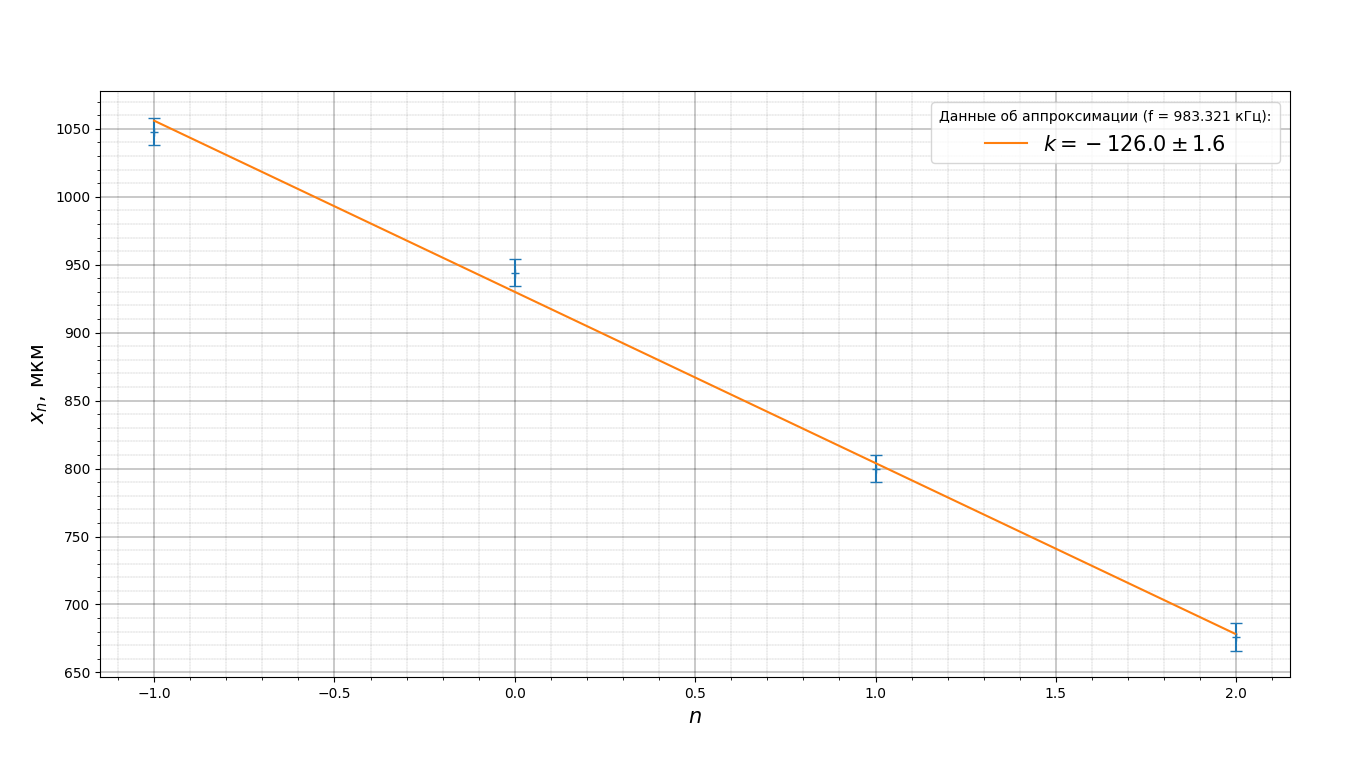
\includegraphics[width=0.8\linewidth]{graph_1}
		\caption{График зависимости координаты от порядка минимума (f = 983.321 кГц)}
		\label{fig:graph1}
	\end{figure}
	\begin{table}[H]
		\centering
		\begin{tabular}{|c|c|c|c|c|c|}
			\hline
			n      & -2   & -1   & 0    & 1    & 2    \\ \hline
			x, мкм & 2.67 & 2.32 & 2.29 & 1.64 & 1.23 \\ \hline
		\end{tabular}
		\caption{Зависимость координаты от порядка минимума (f = 1.137 МГц)}
	\end{table}
	\begin{figure}[H]
		\centering
		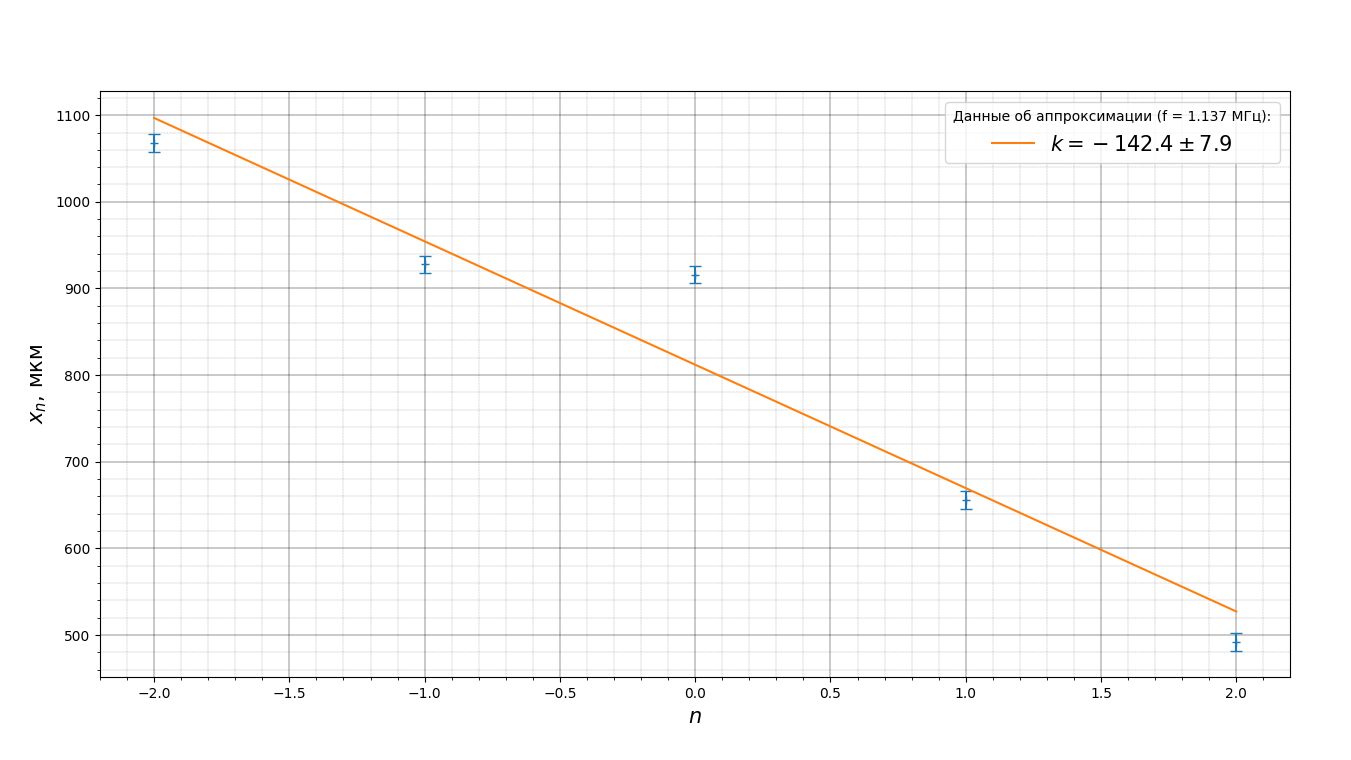
\includegraphics[width=0.8\linewidth]{graph_2}
		\caption{График зависимости координаты от порядка минимума (f = 1.137 МГц)}
		\label{fig:graph2}
	\end{figure}
	\begin{table}[H]
		\centering
		\begin{tabular}{|c|c|c|c|}
			\hline
			n      & -1   & 0    & 1    \\ \hline
			x, мкм & 2.57 & 2.16 & 1.47 \\ \hline
		\end{tabular}
		\caption{Зависимость координаты от порядка минимума (f = 1.9 МГц)}
	\end{table}
	\begin{figure}[H]
		\centering
		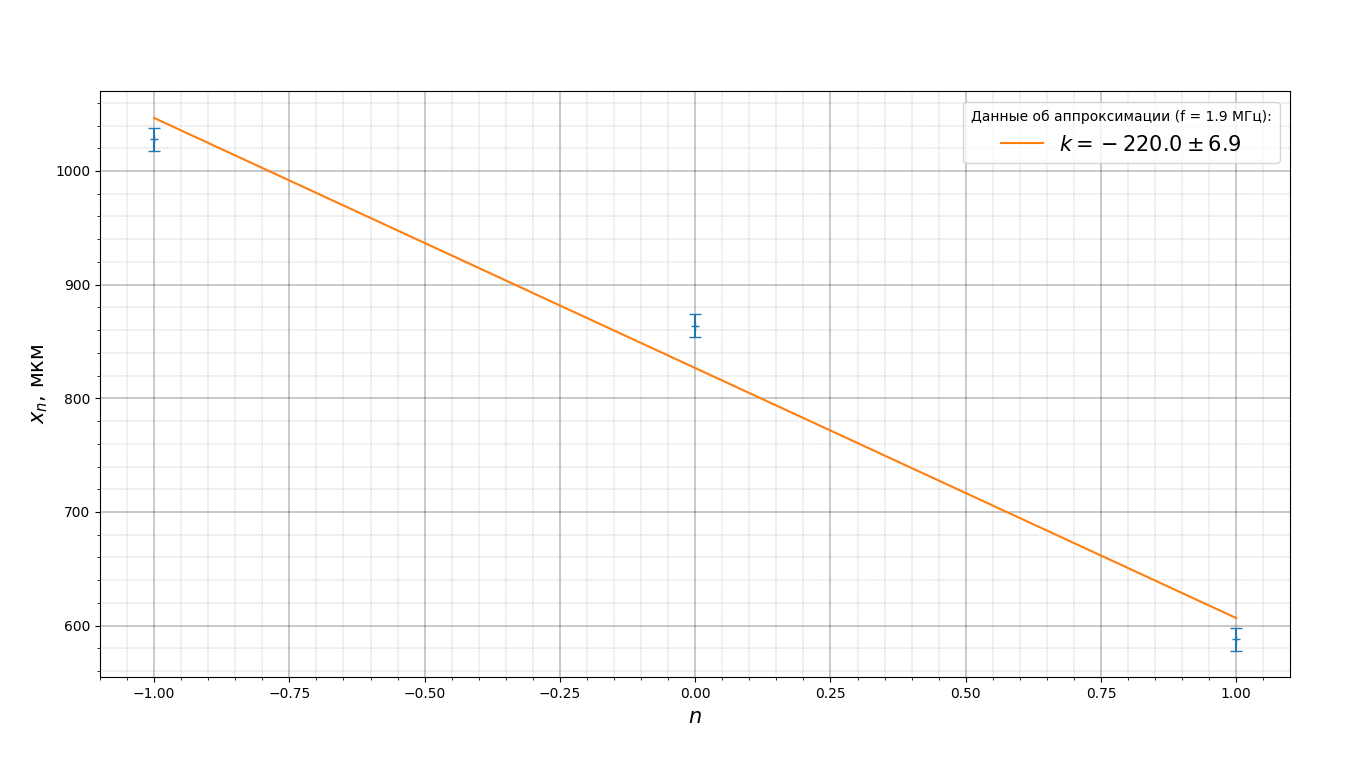
\includegraphics[width=0.8\linewidth]{graph_3}
		\caption{График зависимости координаты от порядка минимума (f = 1.9 МГц)}
		\label{fig:graph3}
	\end{figure}
	Сведем полученные данные в одну таблицу и произведем рассчет скорости распространения волны в жидкости.
	\begin{table}[H]
		\centering
		\begin{tabular}{|c|c|c|c|c|c|c|}
			\hline
			$f$, МГц     & k, мкм     & $\delta k$, мкм & $\Lambda$, мкм & $\delta \Lambda$, мкм & $v$, м/с      &  $\delta v$, м/с  \\ \hline
			0.983 & 126.0 & 1.6     & 1523.8 & 20.3         & 1497.9 & 19.0    \\ \hline
			1.137 & 142.4 & 7.9     & 1348.3 & 75.8         & 1533.0 & 85.2    \\ \hline
			1.900 & 220.0 & 6.9     & 872.7  & 27.3         & 1658.2 & 52.0    \\ \hline
		\end{tabular}
		\caption{Результаты расчета скорости ультразвука}
	\end{table}
	Итого получили для скорости распространения ультразвука в жидкости: $v = 1562 \pm 85.2$ м/с. Полученные значения хорошо сходятся с теоретическими.
	\subsection{Определение скорости ультразвука методом темного поля}
	
	Для наблюдения акустической решетки используется метод темного поля, который заключается в устранении центрального дифракционного максимума с помощью непрозрачного экрана. Схема установки показана на рисунке 6.
	\begin{figure}[H]
		\centering	
		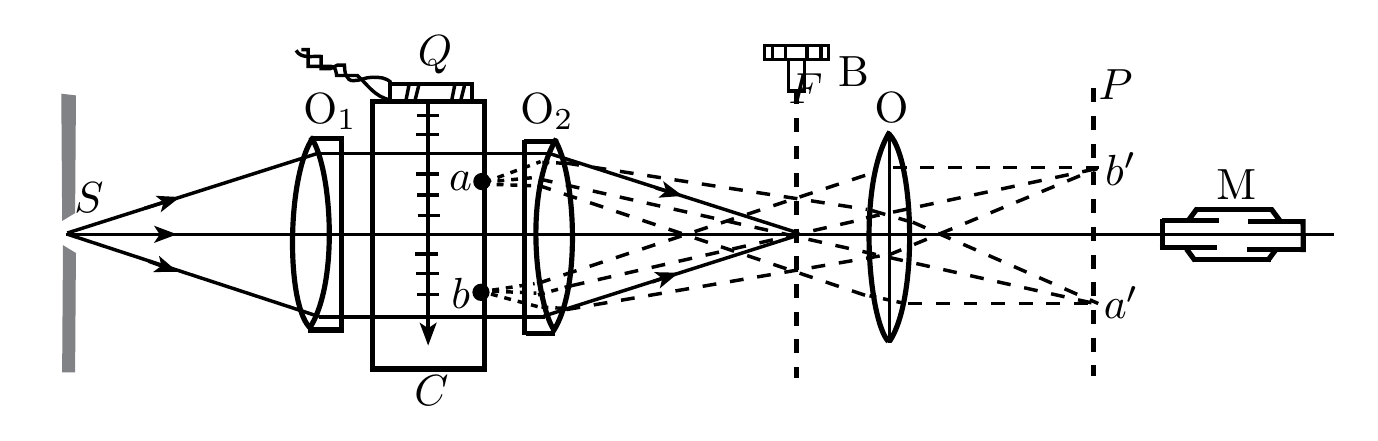
\includegraphics[width=0.7\linewidth]{shema2.png}
		\caption{Схема наблюдения дифракции методом темного поля}
		\label{fig:}
	\end{figure}
	Приставим к задней стенке (для светового луча) кюветы стеклянную пластинку с миллиметровыми делениями; сфокусируем микроскоп на изображение пластинки. Определим цену деления окулярной шкалы микроскопа, совместив ее с миллиметровыми делениями: в 6 делениях миллиметровой шкалы убирается 100 маленьких делений окулярной. Значит, цена деления окулярной шкалы: $ C = $ 0,06 мм.
	
	Без применения метода темного поля звуковая решетка не наблюдается. Закроем нулевой максимум горизонтальной нитью. Таким образом, осевая составляющая фазово-модулированной волны поглощается, а боковые остаются без изменения. Получившееся поле: 
	
	\begin{equation}\label{}
		f(x) = \dfrac{im}{2} e^{i\Omega x} +  \dfrac{im}{2} e^{-i\Omega x} = im \cos \Omega x ; I(x) = m^2 \cos ^2 \Omega x = m^2 \dfrac{1 + \cos ^2 2 \Omega x}{2}
	\end{equation}
	
	Отсюда получаем, что расстояние между темными полосами есть $ \Lambda/2 $.
	
	Проведем измерение длины ультразвуковой волны, приняв ошибку равной цене деления окулярной шкалы. В таблице 6 содержатся количество маленьких делений окулярной шкалы N (цена деления $ C = 0,06 $), соответствующее $ n $ темным полосам акустической решетки.
	Формулы для расчета длины волны ультразвука $ \Lambda $ и скорости распространения $ v $ в воде:
	\begin{equation}\label{}
		\Lambda/2  = NC/(n - 1),  \qquad v = \nu\Lambda
	\end{equation}
	
	Расчеты также приведены в таблице 6. Ошибка при таком определении скорости звука больше, чем в первой части работы, и
	составляет около 5\%. Сами значения тоже получились больше.
	\begin{center}
		\begin{tabular}{|c|c|c|c|c|c|}
			\hline
			$\nu$, Мгц & Кол.дел. $N$ & Кол. т.полос $n$ & $\Lambda$, мм & $v$, $10$ м/с & $\Delta v$, $10$ м/с\\
			\hline
			1,220&150&15&1,29&157&7\\
			\hline
			1,259&150&16&1,20&151&8\\
			\hline
			1,271&175&18&1,24&157&8\\
			\hline
		\end{tabular}
	\end{center}
		Вычисление длины ультразвуковой волны $ \Lambda $ и скорости распространения ее в воде $ v $ методом темного поля
	\section{Выводы}
	В работе измерили скорость распространения ультразвука в воде. Получили: $v = 1562 \pm 85.2$ м/с, табличное значение: $v = 1500$ м/с. Полученное значение совпадает с теоретическим в пределах погрешности.\\
	Значение полученное при помощи метода темного поля совпадает с теоретическим
\end{document}